\documentclass{article}
\usepackage[utf8]{inputenc}

\title{Projeto Final}
\author{Nuno Gonçalves, 96557\\
Afonso Azenha, 96502}
\date{Janeiro 2020}

\usepackage{natbib}
\usepackage{graphicx}
\usepackage{blindtext}
\usepackage{hyperref}

\begin{document}

\maketitle

\section{Tema.}
O trabalho escolhido foi: Sistema horizontal constituído por uma massa ligada a uma mola e outra massa que colide com ela e com uma parede.

\begin{figure}[h!]
\centering
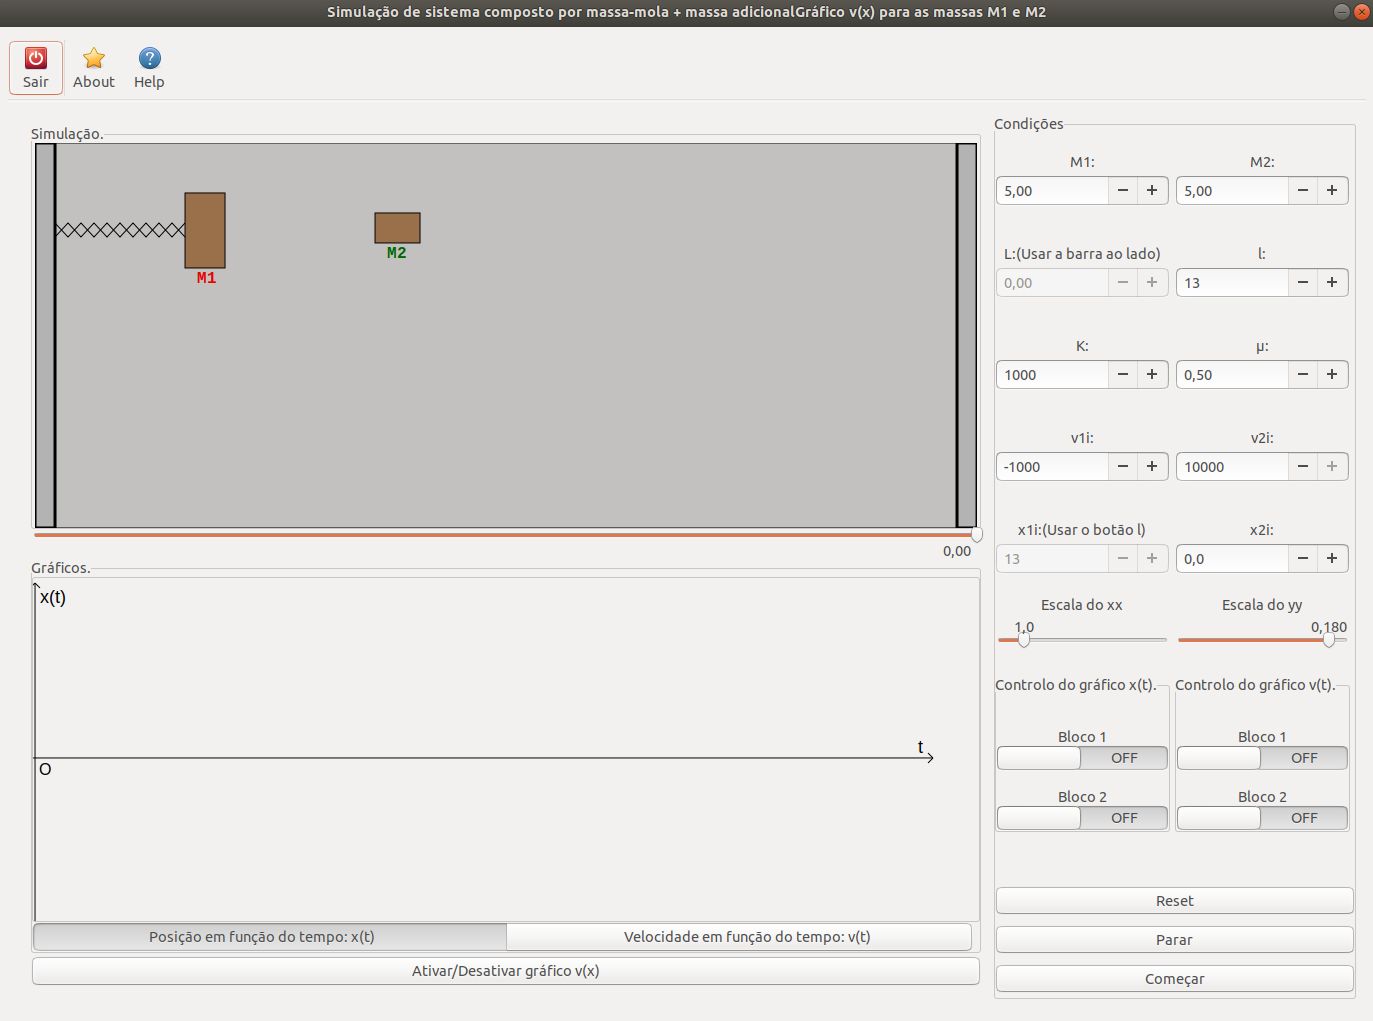
\includegraphics[scale=0.30]{FINAL.png}
\caption{Janela do Programa}
\label{fig:Programa}
\end{figure}

\section{Equações.}
Uma vez que se trata de um oscilador harmónico amortecido calculámos, numericamente, usando  o  método  de Euler-Cromer, a solução da equação diferencial: 
\centerline{$m$ $\frac{d^2x}{dt^2}$ + $\mu$ $\frac{dx}{dt}$ + $k$ ${x}$ = 0};\\
Foram também usadas as fórmulas da colisão elástica (conservação da energia cinética e do momento linear) entre dois corpos A e B:\\
\centerline{V\textsubscript{Af}=($\frac{m\textsubscript{A}-m\textsubscript{B}}{m\textsubscript{A}+m\textsubscript{B}}$)V\textsubscript{Ai}+($\frac{2m\textsubscript{B}}{m\textsubscript{A}+m\textsubscript{B}}$)V\textsubscript{Bi}};\\
\centerline{V\textsubscript{Bf}=($\frac{2m\textsubscript{A}}{m\textsubscript{A}+m\textsubscript{B}}$)V\textsubscript{Ai}+($\frac{m\textsubscript{B}-m\textsubscript{A}}{m\textsubscript{A}+m\textsubscript{B}}$)V\textsubscript{Bi}};\\

\section{Objetivos.}
Com este projeto pretende-se mostrar o movimento de uma massa-mola e uma massa que colidem entre si e com paredes elasticamente. Para melhor compreensão do movimento, na janela é possível a observação de gráficos posição-tempo, velocidade-tempo e velocidade-posição.

\section{Funcionamento do Programa.}
Ao executar o programa é automaticamente aberta uma janela com condições iniciais pré-definidas. Para começar o movimento com estas condições basta clicar no botão "Começar". Caso contrário, pode escolher as variáveis ao seu gosto. As condições são\hypertarget{mylink}{\textbf{[1]}}:
\begin{enumerate}
\item $m$\textsubscript{1} - Massa do Corpo 1;
\item $m$\textsubscript{2} - Massa do Corpo 2;
\item L\textsubscript{0} - Distância entre as duas paredes (pode ajustar este parâmetro através da escala que se encontra por debaixo do desenho da Simulação);
\item $\ell$\textsubscript{0} - Comprimento inicial da mola (tendo em conta que o comprimento natural da mola é 7);
\item $k$ - Constante de elasticidade;
\item $\mu$ - Constante de amortecimento (afeta o movimento do corpo 1);
\item $v$\textsubscript{1i} - Velocidade inicial do bloco 1;
\item $v$\textsubscript{2i} - Velocidade inicial do bloco 2;
\item $x$\textsubscript{1i} - Posição inicial do bloco 1 (esta será automaticamente alterada com a
alteração do l (comprimento inicial da mola);
\item $x$\textsubscript{2i} - Posição inicial do bloco 2;
\end{enumerate}

No topo da janela do programa pode encontrar o botão de sair, o de informação ("About") e o de ajuda ("Help") onde encontrará breves informações sobre a execução do programa.No canto superior esquerdo encontra-se a simulação, logo debaixo os gráficos e à sua direita o controlo da simulação e dos gráficos.
\subsection {Frame Simulação:}
No desenho da simulação encontrará uma barra horizontal que permite ajustar a distância entre as duas paredes.
\subsection {Frame Gráficos:}
Na frame dos gráficos encontram-se todos os gráficos disponibilizados, onde o gráfico posição-tempo e velocidade-tempo podem ser visualizados alternadamente com os botões correspondentes e o gráfico velocidade-posição está associado a um botão que abrirá uma janela para a sua visualização\hyperlink{mylink3}{[3]} (onde terá as mesmas ferramentas de controlo como as dos restantes gráficos). As ferramentas para a alteração da escala e a visibilidade de cada bloco podem ser encontradas na frame das Condições\hyperlink{mylink2}{[2]}. 
\subsection{Frame das condições:}
Aqui encontrará todas as condições iniciais que pode alterar, faladas anteriormente \hyperlink{mylink}{[1]}.\\
Adicionalmente\hypertarget{mylink2}{\textbf{[2]}}, encontrará as ferramentas indicadas com "Escala do xx" e "Escala do yy", que permitirão aumentar ou diminuir as escalas dos eixos do gráfico. Para além disto, terá a possibilidade de esconder o gráfico de qualquer um dos blocos se assim desejar.\\
Por fim, terá os botões de controlo da simulação:\\ 
O botão \textbf{"Reset"} que permite colocar as condições atuais nas condições pre-definidas e colocar os blocos nas suas posições iniciais, parando o programa dando a oportunidade ao utilizador de ajustar de novo os parâmetros.\\
O botão \textbf{"Parar"} que permite parar a simulação.\\
E, por fim, o botão \textbf{"Começar"} que permite começar a simulação com as condições escolhidas.


\begin{figure}[h!]
\centering
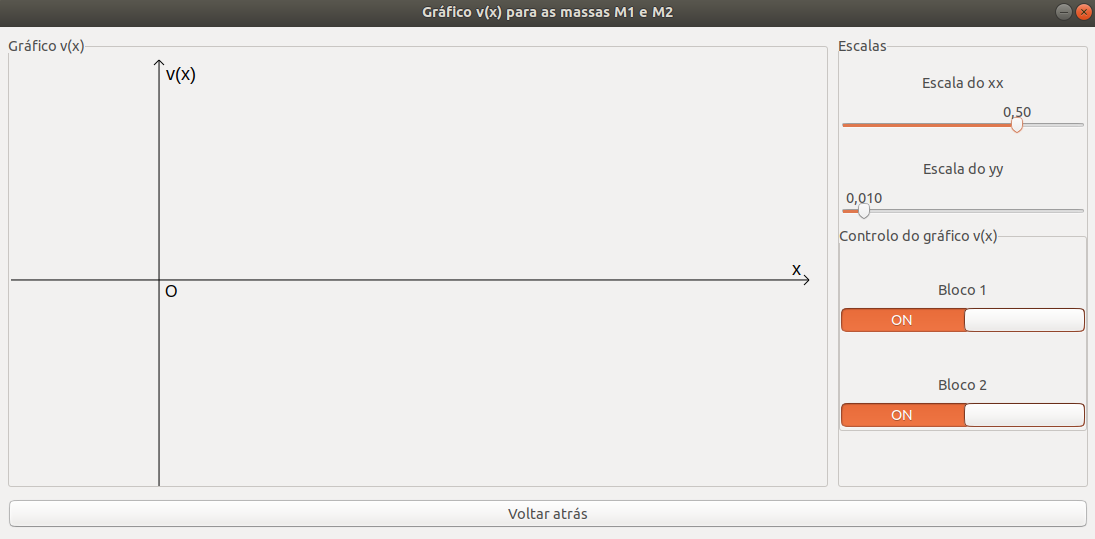
\includegraphics[scale=0.30]{FINAL2.png}
\caption{Gráfico V(x).\hypertarget{mylink3}{[3]}}
\label{fig:Programa}
\end{figure}

\end{document}
